\newcommand\WWtil{{\tilde{\mathbf{W}}}}
\newcommand\hh{{\boldsymbol{\mathit{h}}}}

\chapter{Random Walks}

\sloppy

Today, we talk about random walks on graphs and how the spectrum of the Laplacian guides convergence of random walks. We start by giving the definition of a random walk on a weighted graph $G=(V,E,w)$.

\section{A Primer on Random Walks}

\paragraph{Random Walk Basics.} We call a random sequence of vertices $v_0, v_1, \dots$ a \emph{random walk} on $G$, if $v_0$ is a vertex in $G$ chosen according to some probability distribution $\pp_0 \in \mathbb{R}^V$; and for any $t \geq 0$, we have 
\[
\mathbb{P}[v_{t+1} = v \; | v_t = u] = \begin{cases}
    w(u,v)/\dd(u) & \text{if } \{u,v\} \in E,\\
    0 & \text{otherwise}.
\end{cases}
\]

\begin{figure}[!ht]
    \centering\label{fig:randomWalkSimple}
    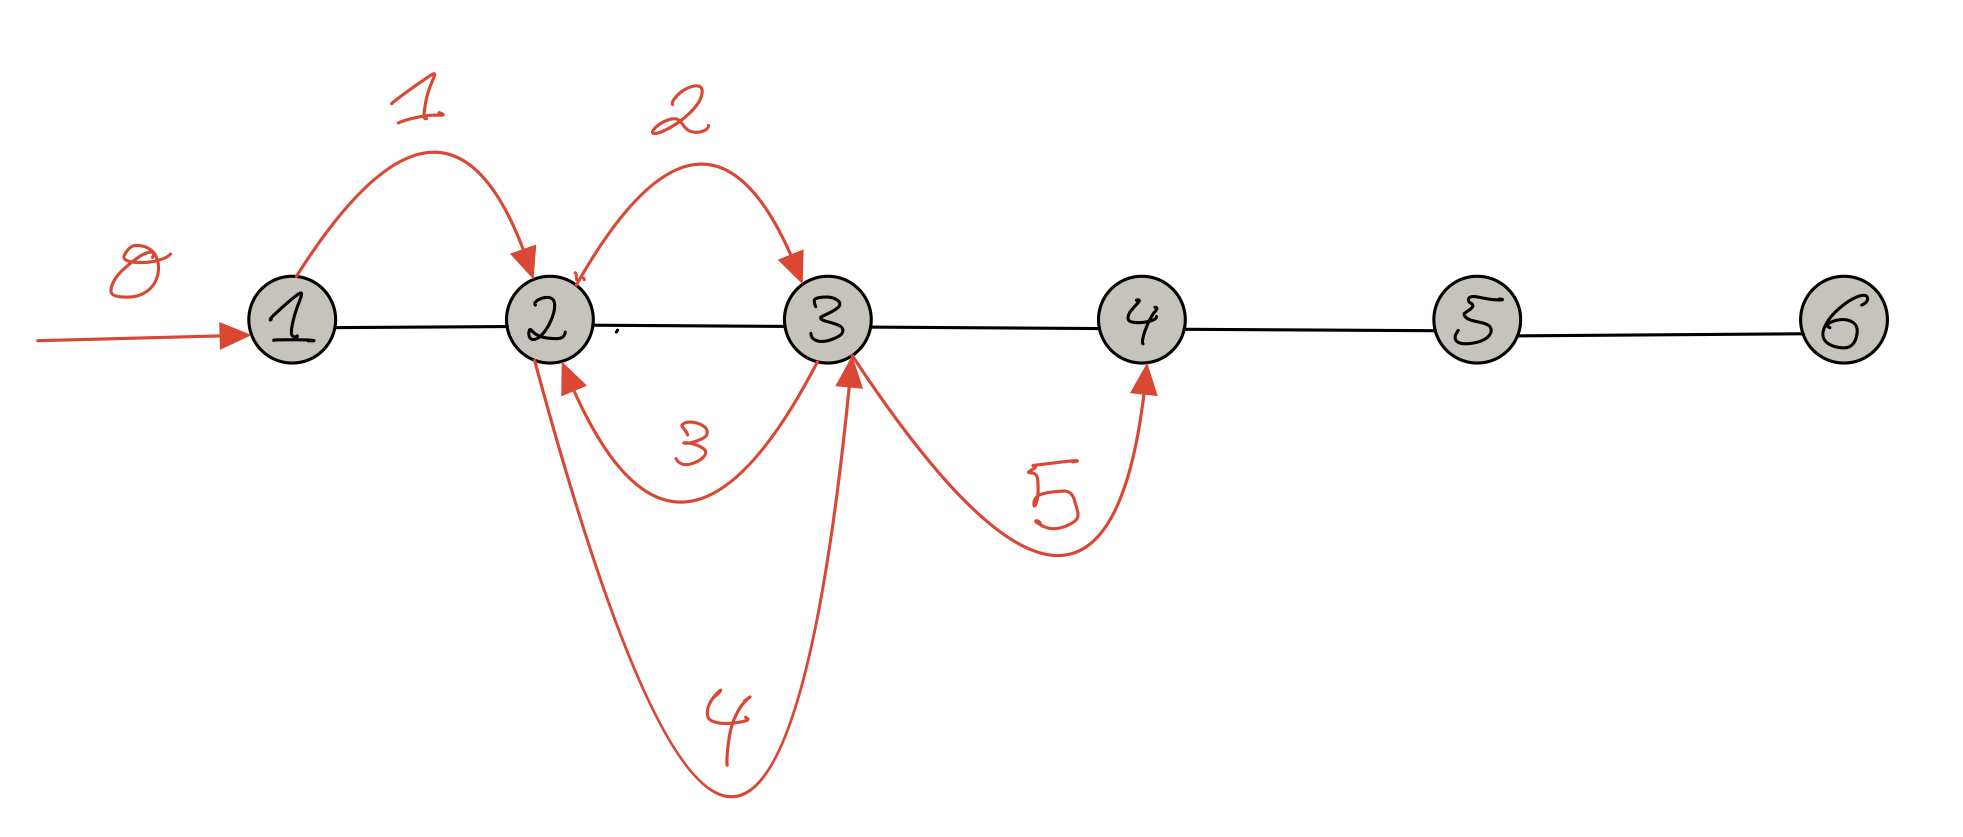
\includegraphics[scale=0.4]{fig/lec_RandomWalks_fig1.png}
    \caption{A (possibly random) walk where the red edges indicate the edges that the particle moves along. Here the walk visits the vertices $v_0 = 1, v_1 = 2, v_2 = 3, v_3 = 2, v_4 = 3, v_5 = 4$.}
    \label{fig:my_label}
\end{figure}

To gain some intuition for the definition,  assume first that the graph $G$ is undirected. Consider a {\color{red}particle} that is placed at a random vertex $v_0$ initially. Then at each step the particle is moved to a neighbor of the current vertex it is resting at, where the neighbor is chosen uniformly at random. 

If the graph is weighted, then instead of choosing a neighbor $v_{t+1}$ of a vertex $v_t$ at each step uniformly at random, one chooses a neighbor $v$ of $v_t$ with probability $w(v,v_t)$ divided by the degree $\dd(v_t)$.

\paragraph{The Random Walk Matrix.} We now define the random walk matrix $\WW$ by
\[
    \WW = \AA \DD^{-1}
\]
and observe that for all vertices $u,v \in V$ (and any $t$), we have that 
\[
\WW_{vu} = \begin{cases}
    w(u,v)/\dd(u) & \text{if } \{u,v\} \in E,\\
    0 & \text{otherwise}.
\end{cases}
\]
Thus, $\WW_{vu} = \mathbb{P}[v_{t+1} = v \; | v_t = u]$ (for any $t$). 

Therefore, $W \vecone_u$ is the distribution over the vertices that the random walk visits them at the next time step, given that it currently is at $u$. More generally, we can now compute the distribution $\pp_1$ over the vertices that they are visited at time $1$ by $\WW \pp_0$, the distribution $\pp_2$ by $\WW \pp_1 = \WW ( \WW \pp_0)$ and so on. Another way of writing this is $\pp_t = \WW^t \pp_{0}$.

\section{Convergence Results for Random Walks}

In this first part of the chapter, we are interested mostly in convergence of random walks that is the two questions:
\begin{itemize}
	\item How does a random walk behave after a large number of steps are taken? 
	\item How many steps does it take asymptotically until the random walk behaves as if an infinite number of steps were taken?
\end{itemize}

To start shedding some light on these questions, we introduce stationary distributions.

\paragraph{Stationary Distribution.} We call a distribution $\ppi \in \mathbb{R}^V$, a \emph{stationary distribution} if $\WW\ppi = \ppi$. That is $\ppi$ is an eigenvector of $\WW$ associated with eigenvalue $1$. It turns out such a stationary distribution always exists.

\begin{lemma}\label{lma:thereExistsStationaryDistr}
Every graph $G$ has a stationary distribution.
\end{lemma}
\begin{proof}
Let $\ppi = \frac{\dd}{\vecone^\trp\dd}$. Clearly, we have that $\|\ppi\|_1 = \sum_{v \in V} \dd(v)/\vecone^\trp\dd = \frac{1}{\vecone^\trp\dd} \sum_{v \in V} \dd(v) = 1$, so $\ppi$ is indeed a distribution. Further note that
\[
\WW \ppi = \AA \DD^{-1} \cdot  \frac{\dd}{\vecone^\trp\dd} = \frac{\AA \vecone}{\vecone^\trp \dd} = \frac{\dd}{\vecone^\trp \dd} = \ppi.
\]
\end{proof}

For many graphs one can show that for $t \to \infty$, we have that $\pp_t \to \ppi$, i.e. that independent of the starting distribution $\pp_0$, the random walk always converges to distribution $\ppi$. 

Unfortunately, this is not true for all graphs: take the graph of two vertices connected by a single edge with $\pp_0$ being $1$ at one vertex and $0$ at the other. 

\subsection{Making Random Walks Lazy}

\paragraph{Lazy Random Walks.} Luckily, we can overcome this issue by using a \emph{lazy random walk}. A lazy random walk behaves just like a random walk, however, at each time step, with probability $\frac{1}{2}$ instead of transitioning to a neighbor, it simply stays put. We give the lazy random walk matrix by
\[
 \WWtil = \frac{1}{2}\II + \frac{1}{2} \WW = \frac{1}{2}\left(\II + \AA \DD^{-1}\right).
\]
It is not hard to see that the stationary distribution $\ppi$ for $\WW$, is also a stationary distribution for $\WWtil$.

\begin{figure}[!ht]
    \centering\label{fig:randomLazyWalkSimple}
    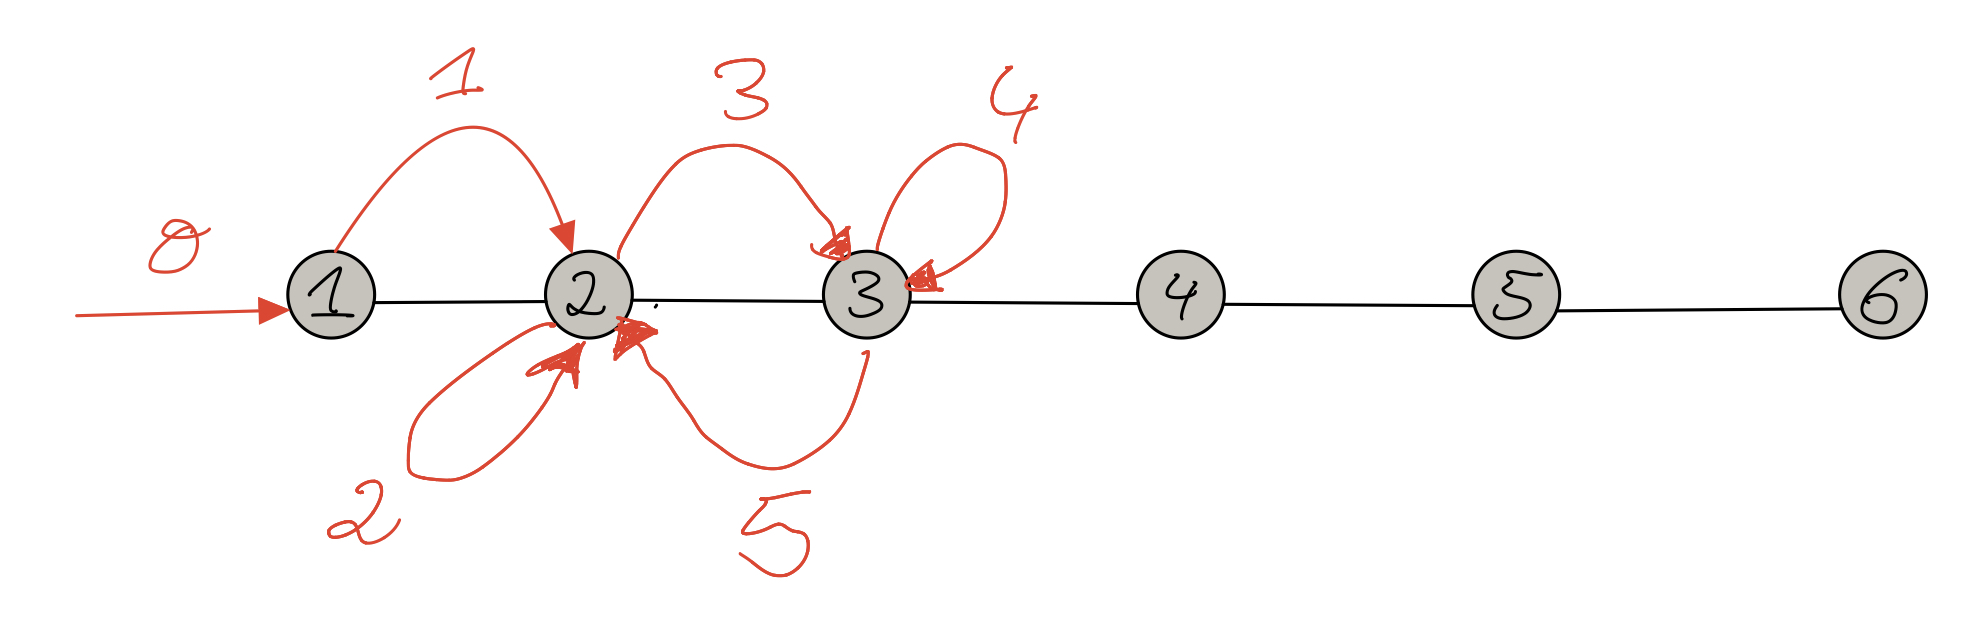
\includegraphics[scale=0.2]{fig/lec_RandomWalks_fig2.jpg}
    \caption{A lazy random walk where the red edges indicate the edges that the particle moves along. Here the lazy walk visits the vertices $v_0 = 1, v_1 = 2, v_2 = 2, v_3 = 3, v_4 = 3, v_5 = 2$.}
    \label{fig:my_label}
\end{figure}

\paragraph{Lazy Random Walks and the Normalized Laplacian.} Recall that we defined $\NN = \DD^{-1/2}\LL \DD^{-1/2} = \II - \DD^{-1/2}\AA \DD^{-1/2} \iff \DD^{-1/2}\AA \DD^{-1/2} = \II - \NN$. We can therefore derive
\begin{align*}
    \WWtil &= \frac{1}{2}\II + \frac{1}{2} \AA \DD^{-1}\\
    &= \frac{1}{2}\II + \frac{1}{2} \DD^{1/2}\DD^{-1/2} \AA \DD^{-1/2}\DD^{-1/2}\\
     &= \frac{1}{2}\II + \frac{1}{2} \DD^{1/2}(\II - \NN) \DD^{-1/2}\\
    &= \frac{1}{2}\II + \frac{1}{2} \DD^{1/2}\II \DD^{-1/2} - \frac{1}{2} \DD^{1/2}\NN \DD^{-1/2}\\
    &= \II - \frac{1}{2} \DD^{1/2}\NN \DD^{-1/2}
\end{align*}

We will now start to reason about the eigenvalues and eigenvectors of $\WWtil$ in terms of the normalized laplacian $\NN$ that we are already familiar with.

For the rest of the lecture, we let $\nu_1 \leq \nu_2 \leq \dots \leq \nu_n$ be the eigenvalues of $\NN$ associated with the orthogonal eigenvectors $\ppsi_1, \ppsi_2, \dots, \ppsi_n$ where we know that such eigenvectors exist by the Spectral Theorem. We note in particular that from the last lecture, we have that $\ppsi_1 = \frac{\dd^{1/2}}{(\vecone^{\trp} \dd)^{1/2}}$ (see Equation \ref{eq:plugInNormalizedVector} where we added a normalization such that $\ppsi_1^{\trp} \ppsi_1 = 1$).

\begin{lemma}\label{lma:correspondenceEigenvectorWalkMatrix}
For the $i^{th}$ eigenvalue $\nu_i$ of $\NN$ associated with eigenvector $\bm{\psi}_i$, we have that $\WWtil$ has an eigenvalue of $(1 - \frac{1}{2}\nu_i)$ associated with eigenvector $\DD^{1/2} \ppsi_i$.
\end{lemma}
\begin{proof}
The proof is by straight-forward calculations
\begin{align*}
    \WWtil \DD^{1/2} \bm{\psi}_i &= (\II - \frac{1}{2} \DD^{1/2}\NN \DD^{-1/2})\DD^{1/2} \bm{\psi}_i \\ &= \DD^{1/2} \bm{\psi}_i - \frac{1}{2} \DD^{1/2}\NN \bm{\psi}_i \\
    &=\DD^{1/2} \bm{\psi}_i - \frac{1}{2} \DD^{1/2}\bm{\psi}_i \nu_i = \DD^{1/2} \bm{\psi}_i (1 - \frac{1}{2}\nu_i).
\end{align*}
\end{proof}

\begin{corollary}
Every eigenvalue of $\WWtil$ is in $[0,1]$.
\end{corollary}
\begin{proof}
Recall that $\LL \pleq 2\DD$ which implies that $\NN \pleq 2 \II$. But this implies that every eigenvalue of $\NN$ is in $[0,2]$. Thus, using Lemma \ref{lma:correspondenceEigenvectorWalkMatrix}, the corollary follows.
\end{proof}

\subsection{Convergence of Lazy Random Walks}

We have now done enough work to obtain an interesting result. We can derive an alternative characterization of $\pp_t$ by expanding $\pp_0$ along an orthogonal eigenvectors basis and then we can repeatedly apply $\WWtil$ by taking powers of the eigenvalues. 

Unfortunately, $\WWtil$ is not symmetric so its eigenvectors are not necessarily orthogonal. Instead, we use a simple trick that allows to expand along the eigenvectors of $\NN$
\begin{align}\label{eq:definitionOfAlphaForWalks}
     \forall i, \ppsi_i^{\trp} \DD^{-1/2} \pp_0 = \alpha_i \iff \DD^{-1/2} \pp_0 = \sum_{i=1}^n \alpha_i \ppsi_i \iff  \pp_0 = \sum_{i=1}^n \alpha_i \DD^{1/2} \ppsi_i.
\end{align}
The above equivalences are best understood if you start from the middle. To get to the left side, you need to observe that multiplying both sides by $\ppsi_i^{\trp}$ cancels all terms $\ppsi_j$ with $j \neq i$ in the sum by orthogonality. To get the right hand side expression, one can simply left-multiply by $\DD^{1/2}$. Technically, we have to show that $\DD^{-1/2}\pp_0$ lives in the eigenspace of $\NN$ but we leave this as an exercise.

This allows us to express a right multiplication by $\WWtil$ as
\[
    \pp_1 = \WWtil \pp_0 = \sum_{i=1}^n \alpha_i \WWtil \DD^{1/2} \ppsi_i = \sum_{i=1}^n \alpha_i \left(1-\frac{\nu_i}{2}\right) \DD^{1/2} \ppsi_i.
\]
And as promised, if we apply $\WWtil$, the lazy random walk operator, $t$ times, we now obtain
\begin{align}\label{eq:distributionRandomWalkTSteps}
    \pp_t = \sum_{i=1}^n \alpha_i \left(1-\frac{\nu_i}{2}\right)^t \DD^{1/2} \ppsi_i = \alpha_1 \DD^{1/2} \ppsi_1 + \sum_{i=2}^n \alpha_i \left(1-\frac{\nu_i}{2}\right)^t \DD^{1/2} \ppsi_i.
\end{align}
where we use in the last equality that $\nu_1 = 0$. Using this simple characterization, we immediately get that $\pp_t \to \ppi$ if $\nu_i > 0$ for all $i \geq 2$ (which is exactly when the graph is connected as you will prove in an exercise). To see this, observe that as $t$ grows sum vanishes. We have that
\[
    \lim_{t \to \infty} \pp_t = \alpha_1 \DD^{1/2} \ppsi_1 = \ppi.
\]
where we used in the equality that $\DD^{1/2} \ppsi_1 = \frac{\dd }{(\vecone^{\trp} \dd)^{1/2}}$ and the value of $\alpha_1$ (from \ref{eq:definitionOfAlphaForWalks}).

\begin{theorem}
For any connected graph $G$, we have that the lazy random walk converges to the stationary distribution of $G$.
\end{theorem}

\subsection{The Rate of Convergence}

Let us now come to the main result that we want to prove this lecture. 

\begin{theorem}
For any $\pp_0$, at any time step $t$, we have for $\pp_t = \WWtil^t \pp_0$ that
\[
\| \pp_t - \ppi \|_{\infty}  \leq e^{-\nu_2 \cdot t/2} \sqrt{n} 
\]
\end{theorem}

Instead of proving the theorem above, we prove the lemma below which gives point-wise convergence. This makes it more convenient to derive a proof and it is not hard to deduce the theorem above as a corollary.

\begin{lemma}
For all $a,b \in V$, and any time step $t$, we have for $\pp_0 = \vecone_a$ and $\pp_t = \WWtil^t \pp_0$ that
\[
  |\pp_t(b) - \ppi(b)| \leq e^{-\nu_2 \cdot t/2} \sqrt{\dd_b/\dd_a} 
\]
\end{lemma}

From Equation \ref{eq:distributionRandomWalkTSteps}, we obtain that
\begin{align}\label{eq:piecewiseDistribution}
    \pp_t(b) - \ppi(b) &= \vecone_b^\trp(\pp_t - \ppi) = \vecone_b^\trp\left( \sum_{i=2}^n \alpha_i \left(1-\frac{\nu_i}{2}\right)^t \DD^{1/2} \ppsi_i \right)
    \\ & =   \sum_{i=2}^n \alpha_i \left(1-\frac{\nu_i}{2}\right)^t \vecone_b^\trp\DD^{1/2} \ppsi_i
    \leq \left(1-\frac{\nu_2}{2}\right)^t \cdot \sum_{i=2}^n \alpha_i  \vecone_b^\trp\DD^{1/2} \ppsi_i
\end{align}
Taking the absolute value on both sides, we obtain that
\begin{align*}\small
|\pp_t(b) - \ppi(b)|
&\leq \left(1-\frac{\nu_2}{2}\right)^t\sum_{i=2}^n \left|\alpha_i  \vecone_b^\trp\DD^{1/2} \ppsi_i \right|\leq \left(1-\frac{\nu_2}{2}\right)^t \sqrt{\left( \sum_{i=2}^n \alpha_i^2 \right) \left( \sum_{i=2}^n \left(\vecone_b^\trp\DD^{1/2} \ppsi_i \right)^2 \right)}
\end{align*}
where we use Cauchy-Schwarz in the last inequality, i.e. $|\langle \uu, \vv \rangle|^2 \leq \langle \uu, \uu \rangle \cdot \langle \vv, \vv \rangle$. Let us finally bound the two sums:
\begin{itemize}
    \item By \ref{eq:definitionOfAlphaForWalks}, $\sum_{i=2}^n \alpha_i^2 = \sum_{i=2}^n \left(\ppsi^\trp_i \DD^{-1/2}\pp_0 \right)^2 \leq \|\DD^{-1/2}\pp_0\|_2^2 =  \|\DD^{-1/2}\vecone_a\|_2^2 = 1/\dd_a$.
    \item Finally, we show that $\sum_{i=2}^n \left(\vecone_b^\trp\DD^{1/2} \ppsi_i \right)^2 \leq \sum_{i=1}^n \left(\vecone_b^\trp\DD^{1/2} \ppsi_i \right)^2 = \|\DD^{1/2}\vecone_b\|_2^2 = \dd_b$ (we only show the first equality, the other inequalities are straight-forward). We first expand the vector $\DD^{1/2}\vecone_b$ along the eigenvectors using some values $\beta_i$ defined
    \[
        \DD^{1/2}\vecone_b = \sum_{i=1}^n \beta_i \ppsi_i \iff  \ppsi_i^\trp \DD^{1/2}\vecone_b = \beta_i \iff  \vecone_b^\trp \DD^{1/2}\ppsi_i= \beta_i  
    \]
    We used orthogonality to get the first equivalence, and then just take the transpose to get the second. We can now write
    \[
    \|\DD^{1/2}\vecone_b\|_2^2 = (\DD^{1/2}\vecone_b)^{\trp} (\DD^{1/2}\vecone_b) = \left(\sum_{i=1}^n \beta_i \ppsi_i^\trp\right) \left(\sum_{i=1}^n \beta_i \ppsi_i\right) = \sum_{i=2}^n \beta_i^2
    \]
    where we again used orthogonality of $\ppsi_i$. The equality then follows by definition of $\beta_i$.
\end{itemize}

Putting everything together (and using $1+x \leq e^x, \forall x \in \mathbb{R}$), we obtain 
\[  
    |\pp_t(b) - \ppi(b)| \leq \left(1-\frac{\nu_2}{2}\right)^t \sqrt{\dd_b/\dd_a} \leq e^{-\nu_2 \cdot t/2} \sqrt{\dd_b/\dd_a} 
\]

\section{Properties of Random Walks}

We now shift our focus away from convergence of random walks and consider some interesting properties of random walks. Here, we are no longer interested in lazy random walks, although all proofs can be straight-forwardly adapted. While in the previous section, we relied on computing the second eigenvalue of the Normalized Laplacian efficiently, here, we will discover that solving Laplacian systems, that is finding an $\xx$ such that $\LL\xx = \bb$ can solve a host of problems in random walks.

\subsection{Hitting Times}

One of the most natural questions one can ask about a random walk starting in a vertex $a$ (i.e. $\pp_0 = \vecone_a$) is how many steps it takes to get to a special vertex $s$. This quantity is called the \emph{hitting time} from $a$ to $s$ and we denote it by $H_{a,s} = \inf \{ t \;|\; \vv_t = s \}$. For the rest of this section, we are concerned with computing the expected hitting time, i.e. $\mathbb{E}[H_{a,s}]$.

It turns out, that it is more convenient to compute \emph{all} expected hitting times $H_{a,s}$ for vertices $a \in V$ to a fixed $s$. We denote by $\hh \in \mathbf{R}^V$, the vector with $\hh_a = \mathbb{E}[H_{a,s}]$. We now show that we can compute $\hh$ by solving a Laplacian system $\LL \hh = \bb$. We will see later in the course that such systems (spoiler alert!) can be solved in time $\tilde{O}(m)$, so this will imply a near-linear time algorithm to compute the hitting times.

\paragraph{Hitting Time and the Random Walk Matrix.} Let us first observe that if $s = a$, then the answer becomes trivially $0$, i.e. $\hh_s = 0$. 

We compute the rest of the vector by writing down a system of equations that recursively characterizes $\hh$. Observe therefore first that for any $a \neq s$, we have that the random walks starting at $a$ will next visit a neighbor $b$ of $a$. If the selected neighbor $b = s$, the random walks stops; otherwise, the random walks needs in expectation $\mathbb{E}[H_{b,s}]$ time to move to $s$. 

We can express this algebraically by
\[
\hh_a = 1 + \sum_{a \sim b} \mathbb{P}[v_{t+1} = b \;| v_t = a]  \cdot \hh_b = 1 + \sum_{a \sim b} \frac{w(a,b)}{\dd(a)}  \cdot \hh_b =  1 + (\WW\vecone_a)^{\trp} \hh = 1 + \vecone_a^{\trp} \WW^{\trp} \hh.
\]
Using that $\hh_a = \vecone_a^{\trp} \hh =  \vecone_a^{\trp} \II \hh$, we can rewrite this as 
\[
1 = \vecone_a^\trp (\II - \WW^\trp) \hh.
\]
This gives a system of (linear) equations, that can be neatly summarized by 
\[
\vecone - \alpha \cdot \vecone_s = (\II - \WW^\trp) \hh
\]
where we have an extra degree of freedom in choosing $\alpha$ in formulating a constraint $1 - \alpha = \vecone_s^\trp (\II -\WW^\trp) \hh$. This extra degree of freedom stems from the fact that $n-1$ equations suffice for us to enforce that the returned vector $\xx$ to the system  from the system are indeed the hitting times (possibly shifted by the value assigned to coordinate $t$).

\paragraph{Finding Hitting Times via Laplacian System Solve.} Since we assume $G$ connected, we have that multiplying with $\DD = \DD^\trp$ preserves equality. Further since $\WW = \AA \DD^{-1}$, we obtain
\[
\dd - \alpha \cdot \dd(s) \cdot \vecone_s = (\DD - \AA) \hh.
\]
Defining $\bb = \dd - \alpha \cdot \dd(s) \cdot \vecone_s$, and observing $\LL = \DD - \AA$, we have $\LL\hh = \bb$. 

Finally, we observe that we only have a solution to the above system if and only if $\bb \in \ker(\LL)^\perp =  \Span(\vecone)^\perp$. We thus have to set $\alpha$ such that 
\[
\vecone^{\trp}(\dd - \alpha \cdot \dd(s) \cdot \vecone_s) = \|\dd\|_1 - \alpha \cdot \dd(s) \iff \alpha =  \|\dd\|_1 /\dd(s).
\]
We have now formalized $\LL$ and $\bb$ completely. A last detail that we should not forget about is that any solution $\xx$ to such system $\LL \xx = \bb$ is not necessarily equal $\hh$ but has the property that it is shifted from $\hh$ by the all-ones vector. Since we require $\hh_s = 0$, we can reconstruct $\hh$ from $\xx$ straight-forwardly by subtracting $\xx_s \vecone$.

\begin{theorem}
	Given a connected graph $G$, a special vertex $s \in V$. Then, we can formalize a Laplacian system $\LL \xx = \bb$ (where $\LL$ is the Laplacian of $G$) such that the expected hitting times to $s$ are given by $\hh = \xx - \xx_s \vecone$. We can reconstruct $\hh$ from $\xx$ in time $O(n)$.
\end{theorem}

\paragraph{Hitting Times and Electrical Networks.} Seeing that hitting times can be computed by formulating a Laplacian system $\LL \xx = \bb$. You might remember that in the first lecture, we argued that a system $\LL \xx = \bb$ also solves the problem of routing a demand $\bb$ via an electrical flow with voltages $\xx$. 

Indeed, we can interpret computing expected hitting times $\hh$ to a special vertex $s$ as the problem of computing the electrical voltages $\xx$ where we insert (or more technically correct apply) $\dd(a)$ units of current at every vertex $a \neq s$ and where we remove $\vecone^\trp\dd - \dd(s)$ units of current at the vertex $s$. Then, we can express expected hitting time to some vertex $a$ as the voltage difference to $s$: $\mathbb{E}[H_{a,s}] = \hh_a = \xx_a - \xx_s$.

\subsection{Commute Time}

A topic very related to hitting times are \emph{commute times}. That is for two vertices $a,b$, the commute time is the time in a random walk starting in $a$ to visit $b$ and then to return to $a$ again. Thus, it can be defined $C_{a,b} = H_{a,b} + H_{b,a}$.

\paragraph{Commute Times via Electric Flows.} Recall that expected hitting times have an electric flow interpretation. 

Now, let us denote by $\xx$ a solution to the Laplacian system $\LL \xx = \bb_b$ where the demand is $\bb_b = \dd - \dd^\trp \vecone \cdot \vecone_b \in \ker(\vecone)^\perp$. Recall that we have $\mathbb{E}[H_{z,b}] = \xx_z - \xx_b$ for all $z$. 

Similarly, we can compute voltages $\yy$ to the Laplacian system $\LL \yy = \bb_a$ where $\bb_a = \dd - \dd^\trp \vecone \cdot \vecone_a \in \ker(\vecone)^\perp$. Again, $\mathbb{E}[H_{z,a}] = \yy_z - \yy_a$ for all $z$. Note that, if we revert the flow by negating $\yy$, then we can still compute the hitting time by taking $\mathbb{E}[H_{z,a}] = -(-\yy_z - (-\yy_a)) = -(\yy_a-\yy_z)$.

Thus, inducing voltages $\xx - \yy$ on the graph $G$, we now have by linearity that $\mathbb{E}[C_{a,b}] = \mathbb{E}[H_{a,b}+H_{b,a}] = |\xx_a - \xx_b| + |\yy_a-\yy_b|$. But these voltages are also induced by $\LL (\xx - \yy) = \bb_b - \bb_a = \dd^\trp \vecone (\vecone_a - \vecone_b)$ (again by linearity). That is the flow that routes $\|\dd\|_1$ units of flow from $b$ to $a$.  

\begin{theorem}
	Given a graph $G=(V,E)$, for any two fixed vertices $a,b \in V$, the expected commute time $C_{a,b}$ is given by the voltage difference between $a$ and $b$ for any solution $\zz$ to the Laplacian system $\LL \zz = \|\dd\|_1 \cdot (\vecone_b - \vecone_a)$.
\end{theorem}

We note that the voltage difference between $a$ and $b$ in an electrical flow routing demand $\vecone_b - \vecone_a$ is also called the \emph{effective resistance} $\er(a,b)$. This quantity will play a crucial role in the next roles. In the next lecture, we introduce $\er(a,b)$ slightly differently as the energy required by the electrical flow that routes $\vecone_b - \vecone_a$, however, it is not hard to show that these two definitions are equivalent.

Our theorem can now be restated as saying that the expected commute time $\mathbb{E}[C_{a,b}] = \|\dd\|_1 \cdot \er(a,b)$. This is a classic result.